\documentclass[conference]{IEEEtran}
\IEEEoverridecommandlockouts

\usepackage{amsmath,amssymb,amsfonts}
\usepackage{algorithmic}
\usepackage{graphicx}
\usepackage{textcomp}
\usepackage{xcolor}
\usepackage{biblatex}
\addbibresource{refs.bib}

\def\BibTeX{{\rm B\kern-.05em{\sc i\kern-.025em b}\kern-.08em
    T\kern-.1667em\lower.7ex\hbox{E}\kern-.125emX}}
    
\begin{document}

\title{BPC-PRP Project Doc Template}

\author{\IEEEauthorblockN{1\textsuperscript{st} Given Name Surname}
\IEEEauthorblockA{\textit{dept. name of organization (of Aff.)} \\
\textit{name of organization (of Aff.)}\\
City, Country \\
email address or ORCID}
\and
\IEEEauthorblockN{2\textsuperscript{nd} Given Name Surname}
\IEEEauthorblockA{\textit{dept. name of organization (of Aff.)} \\
\textit{name of organization (of Aff.)}\\
City, Country \\
email address or ORCID}
}

\maketitle

\begin{abstract}
Lorem ipsum dolor sit amet, consectetuer adipiscing elit. Morbi scelerisque luctus velit. Quis autem vel eum iure reprehenderit qui in ea voluptate velit esse quam nihil molestiae consequatur, vel illum qui dolorem eum fugiat quo voluptas nulla pariatur? Vivamus luctus egestas leo. Nulla non arcu lacinia neque faucibus fringilla. Class aptent taciti sociosqu ad litora torquent per conubia nostra, per inceptos hymenaeos. Mauris dolor felis, sagittis at, luctus sed, aliquam non, tellus. Mauris metus. Aliquam erat volutpat. Nullam eget nisl. Fusce wisi. Vestibulum fermentum tortor id mi.
\end{abstract}

\begin{IEEEkeywords}
Robotics, project, BPC-PRP, state-of-the-art
\end{IEEEkeywords}


\section{Introduction}

Vivamus ac leo pretium faucibus. Etiam posuere lacus quis dolor. Donec vitae arcu. Nullam eget nisl. Integer lacinia. Morbi scelerisque luctus velit. Pellentesque pretium lectus id turpis. Aliquam id dolor. Integer pellentesque quam vel velit. Nemo enim ipsam voluptatem quia voluptas sit aspernatur aut odit aut fugit, sed quia consequuntur magni dolores eos qui ratione voluptatem sequi nesciunt.

Class aptent taciti sociosqu ad litora torquent per conubia nostra, per inceptos hymenaeos. In enim a arcu imperdiet malesuada. Donec ipsum massa, ullamcorper in, auctor et, scelerisque sed, est. Vivamus porttitor turpis ac leo. Nam sed tellus id magna elementum tincidunt. Pellentesque arcu. Suspendisse sagittis ultrices augue. Integer vulputate sem a nibh rutrum consequat. Etiam dictum tincidunt diam. Et harum quidem rerum facilis est et expedita distinctio. In rutrum. Cras pede libero, dapibus nec, pretium sit amet, tempor quis. Nam sed tellus id magna elementum tincidunt. Nullam faucibus mi quis velit. Ut enim ad minim veniam, quis nostrud exercitation ullamco laboris nisi ut aliquip ex ea commodo consequat. Maecenas libero. Nulla pulvinar eleifend sem. Curabitur bibendum justo non orci. Maecenas libero. Fusce wisi \cite{kalman1960new}.

\begin{figure}[h]
    \centering
    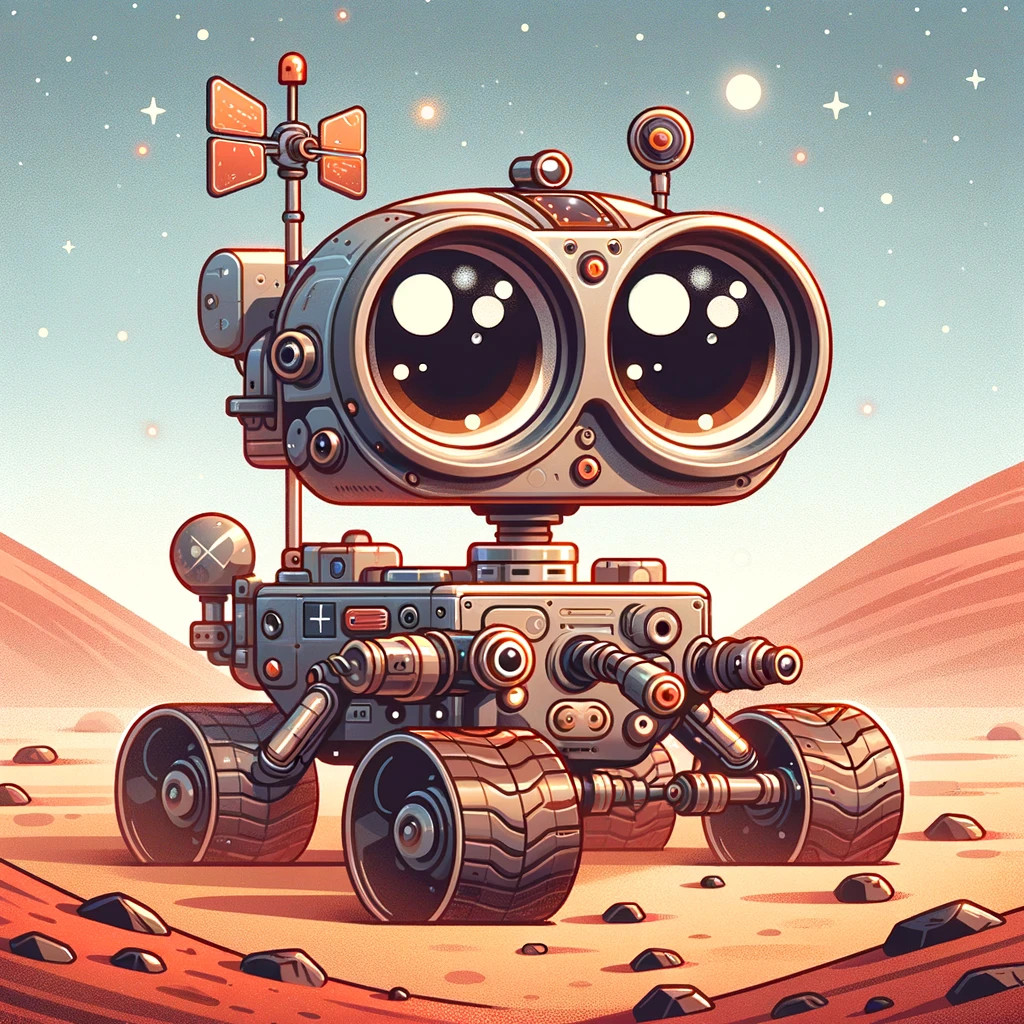
\includegraphics[width=0.45\textwidth]{images/rover.jpg}
    \caption{The mars rover}
    \label{fig:mars_rover}
\end{figure}

Quisque tincidunt scelerisque libero. Cum sociis natoque penatibus et magnis dis parturient montes, nascetur ridiculus mus. Sed vel lectus. Donec odio tempus molestie, porttitor ut, iaculis quis, sem. Temporibus autem quibusdam et aut officiis debitis aut rerum necessitatibus saepe eveniet ut et voluptates repudiandae sint et molestiae non recusandae. Proin in tellus sit amet nibh dignissim sagittis. Nam libero tempore, cum soluta nobis est eligendi optio cumque nihil impedit quo minus id quod maxime placeat facere possimus, omnis voluptas assumenda est, omnis dolor repellendus. Aliquam ornare wisi eu metus. Curabitur bibendum justo non orci. Aliquam erat volutpat. Duis ante orci, molestie vitae vehicula venenatis, tincidunt ac pede. Duis sapien nunc, commodo et, interdum suscipit, sollicitudin et, dolor. Etiam commodo dui eget wisi. Nam quis nulla. Etiam dictum tincidunt diam. \cite{grisetti2010tutorial}

\section{Main Text}

Pellentesque pretium lectus id turpis. Mauris suscipit, ligula sit amet pharetra semper, nibh ante cursus purus, vel sagittis velit mauris vel metus. Sed ut perspiciatis unde omnis iste natus error sit voluptatem accusantium doloremque laudantium, totam rem aperiam, eaque ipsa quae ab illo inventore veritatis et quasi architecto beatae vitae dicta sunt explicabo. In laoreet, magna id viverra tincidunt, sem odio bibendum justo, vel imperdiet sapien wisi sed libero. Mauris elementum mauris vitae tortor. Integer imperdiet lectus quis justo. In sem justo, commodo ut, suscipit at, pharetra vitae, orci. Nullam sit amet magna in magna gravida vehicula. Excepteur sint occaecat cupidatat non proident, sunt in culpa qui officia deserunt mollit anim id est laborum. Mauris tincidunt sem sed arcu.

Praesent dapibus. Suspendisse sagittis ultrices augue. Maecenas sollicitudin. Sed ut perspiciatis unde omnis iste natus error sit voluptatem accusantium doloremque laudantium, totam rem aperiam, eaque ipsa quae ab illo inventore veritatis et quasi architecto beatae vitae dicta sunt explicabo. Suspendisse nisl. Donec vitae arcu. Aenean id metus id velit ullamcorper pulvinar. Phasellus enim erat, vestibulum vel, aliquam a, posuere eu, velit. Suspendisse sagittis ultrices augue. Proin mattis lacinia justo.

Aenean id metus id velit ullamcorper pulvinar. Aliquam erat volutpat. Fusce aliquam vestibulum ipsum. Duis pulvinar. Morbi imperdiet, mauris ac auctor dictum, nisl ligula egestas nulla, et sollicitudin sem purus in lacus. Suspendisse nisl. Maecenas libero. Curabitur vitae diam non enim vestibulum interdum. Nullam dapibus fermentum ipsum. Vivamus porttitor turpis ac leo. Etiam quis quam. Nemo enim ipsam voluptatem quia voluptas sit aspernatur aut odit aut fugit, sed quia consequuntur magni dolores eos qui ratione voluptatem sequi nesciunt. Etiam egestas wisi a erat. Nulla est \cite{thrun2005probabilistic}.

Aliquam ornare wisi eu metus. Maecenas lorem. Aliquam ornare wisi eu metus. Vivamus porttitor turpis ac leo. Donec iaculis gravida nulla. Etiam dictum tincidunt diam. Vestibulum erat nulla, ullamcorper nec, rutrum non, nonummy ac, erat. Aliquam in lorem sit amet leo accumsan lacinia. Integer imperdiet lectus quis justo. Sed vel lectus. Donec odio tempus molestie, porttitor ut, iaculis quis, sem. Vivamus ac leo pretium faucibus. Proin in tellus sit amet nibh dignissim sagittis. Cras elementum. Quisque porta.

Aenean placerat. Nullam at arcu a est sollicitudin euismod. Sed convallis magna eu sem. Temporibus autem quibusdam et aut officiis debitis aut rerum necessitatibus saepe eveniet ut et voluptates repudiandae sint et molestiae non recusandae. Duis ante orci, molestie vitae vehicula venenatis, tincidunt ac pede. Duis viverra diam non justo. In rutrum. Phasellus enim erat, vestibulum vel, aliquam a, posuere eu, velit. In laoreet, magna id viverra tincidunt, sem odio bibendum justo, vel imperdiet sapien wisi sed libero. Maecenas lorem. Etiam quis quam. Maecenas ipsum velit, consectetuer eu lobortis ut, dictum at dui. Sed ac dolor sit amet purus malesuada congue. Etiam neque. Fusce aliquam vestibulum ipsum. Fusce nibh. Etiam dui sem, fermentum vitae, sagittis id, malesuada in, quam. Integer vulputate sem a nibh rutrum consequat.

\begin{figure}[h]
    \centering
    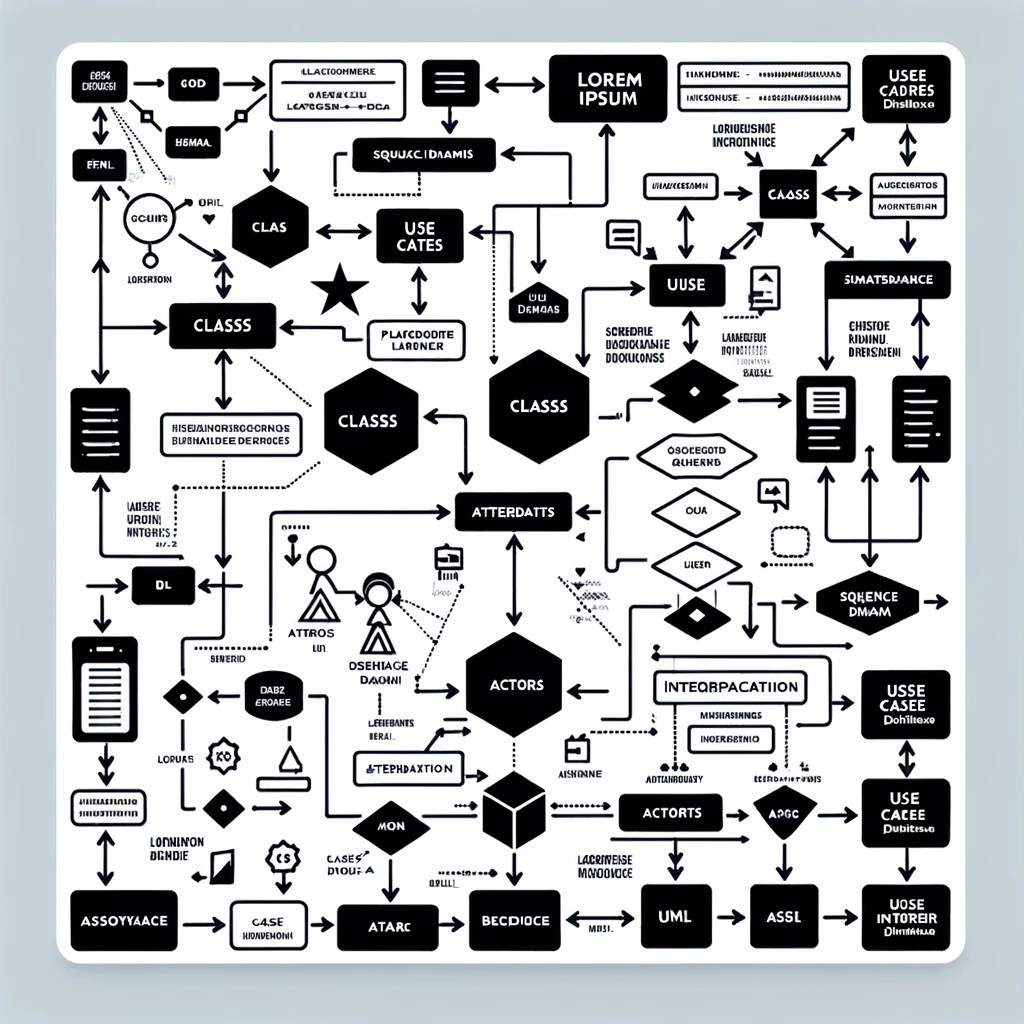
\includegraphics[width=0.45\textwidth]{images/schema.jpg}
    \caption{The schematic}
    \label{fig:schema}
\end{figure}

Phasellus faucibus molestie nisl. Duis viverra diam non justo. Maecenas sollicitudin. Nemo enim ipsam voluptatem quia voluptas sit aspernatur aut odit aut fugit, sed quia consequuntur magni dolores eos qui ratione voluptatem sequi nesciunt. Et harum quidem rerum facilis est et expedita distinctio. Temporibus autem quibusdam et aut officiis debitis aut rerum necessitatibus saepe eveniet ut et voluptates repudiandae sint et molestiae non recusandae. Praesent in mauris eu tortor porttitor accumsan. Duis ante orci, molestie vitae vehicula venenatis, tincidunt ac pede. Aliquam in lorem sit amet leo accumsan lacinia. Phasellus et lorem id felis nonummy placerat. Etiam posuere lacus quis dolor. Integer lacinia. Nullam faucibus mi quis velit. Nunc auctor. Phasellus et lorem id felis nonummy placerat.

Nullam justo enim, consectetuer nec, ullamcorper ac, vestibulum in, elit. Neque porro quisquam est, qui dolorem ipsum quia dolor sit amet, consectetur, adipisci velit, sed quia non numquam eius modi tempora incidunt ut labore et dolore magnam aliquam quaerat voluptatem. Nunc dapibus tortor vel mi dapibus sollicitudin. Pellentesque pretium lectus id turpis. In convallis. Fusce aliquam vestibulum ipsum. Fusce consectetuer risus a nunc. Vestibulum fermentum tortor id mi. Aenean fermentum risus id tortor. Nullam at arcu a est sollicitudin euismod.

Mauris elementum mauris vitae tortor. Aliquam ornare wisi eu metus. Cum sociis natoque penatibus et magnis dis parturient montes, nascetur ridiculus mus. Duis sapien nunc, commodo et, interdum suscipit, sollicitudin et, dolor. Duis ante orci, molestie vitae vehicula venenatis, tincidunt ac pede. Duis viverra diam non justo. Pellentesque sapien. Mauris dolor felis, sagittis at, luctus sed, aliquam non, tellus. Etiam posuere lacus quis dolor. Nulla non lectus sed nisl molestie malesuada. Nullam dapibus fermentum ipsum.

Sed convallis magna eu sem. Suspendisse sagittis ultrices augue. Pellentesque habitant morbi tristique senectus et netus et malesuada fames ac turpis egestas. Sed ut perspiciatis unde omnis iste natus error sit voluptatem accusantium doloremque laudantium, totam rem aperiam, eaque ipsa quae ab illo inventore veritatis et quasi architecto beatae vitae dicta sunt explicabo. Phasellus et lorem id felis nonummy placerat. In laoreet, magna id viverra tincidunt, sem odio bibendum justo, vel imperdiet sapien wisi sed libero. Aliquam erat volutpat. Nullam at arcu a est sollicitudin euismod. Praesent id justo in neque elementum ultrices. Aenean placerat. Nullam lectus justo, vulputate eget mollis sed, tempor sed magna. Aenean fermentum risus id tortor. Nam quis nulla. Aliquam erat volutpat.

Phasellus faucibus molestie nisl. Maecenas lorem. Nulla est. Integer tempor. Itaque earum rerum hic tenetur a sapiente delectus, ut aut reiciendis voluptatibus maiores alias consequatur aut perferendis doloribus asperiores repellat. Vivamus ac leo pretium faucibus. Quisque tincidunt scelerisque libero. Class aptent taciti sociosqu ad litora torquent per conubia nostra, per inceptos hymenaeos. Nullam at arcu a est sollicitudin euismod. In convallis. Nulla turpis magna, cursus sit amet, suscipit a, interdum id, felis. Proin pede metus, vulputate nec, fermentum fringilla, vehicula vitae, justo. Vivamus porttitor turpis ac leo. Etiam dictum tincidunt diam. Donec iaculis gravida nulla. Proin mattis lacinia justo \cite{grisetti2010tutorial}.

Donec quis nibh at felis congue commodo. Nullam sapien sem, ornare ac, nonummy non, lobortis a enim. Nam libero tempore, cum soluta nobis est eligendi optio cumque nihil impedit quo minus id quod maxime placeat facere possimus, omnis voluptas assumenda est, omnis dolor repellendus. Duis bibendum, lectus ut viverra rhoncus, dolor nunc faucibus libero, eget facilisis enim ipsum id lacus. Morbi leo mi, nonummy eget tristique non, rhoncus non leo. Cras elementum. Fusce dui leo, imperdiet in, aliquam sit amet, feugiat eu, orci. Maecenas aliquet accumsan leo. Pellentesque arcu. Vestibulum erat nulla, ullamcorper nec, rutrum non, nonummy ac, erat. Aliquam ante. Etiam quis quam. Phasellus enim erat, vestibulum vel, aliquam a, posuere eu, velit. Proin pede metus, vulputate nec, fermentum fringilla, vehicula vitae, justo. Vestibulum erat nulla, ullamcorper nec, rutrum non, nonummy ac, erat. Mauris dictum facilisis augue. Aenean placerat. Nullam justo enim, consectetuer nec, ullamcorper ac, vestibulum in, elit. Morbi scelerisque luctus velit. Nam sed tellus id magna elementum tincidunt.

\begin{figure}[h]
    \centering
    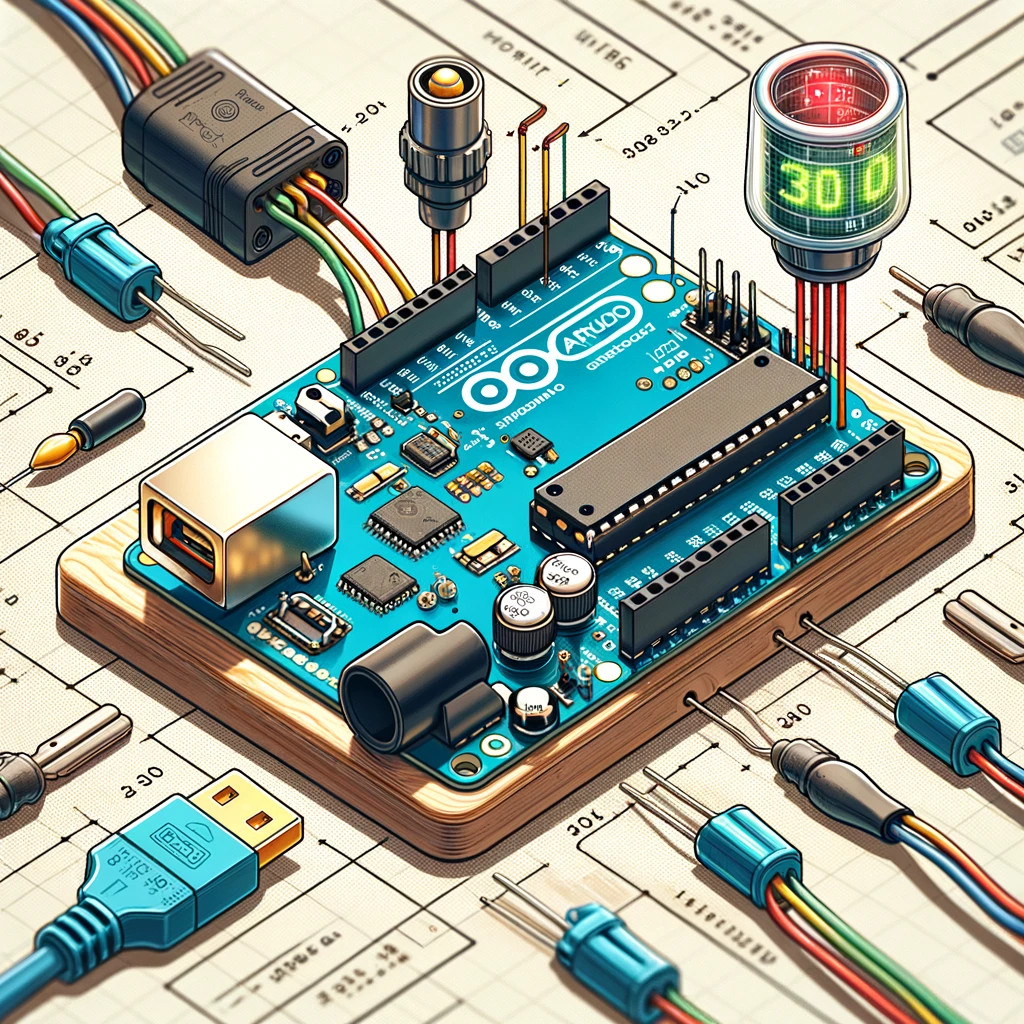
\includegraphics[width=0.45\textwidth]{images/arduino.jpg}
    \caption{Arduino}
    \label{fig:arduino}
\end{figure}

Praesent vitae arcu tempor neque lacinia pretium. Ut enim ad minim veniam, quis nostrud exercitation ullamco laboris nisi ut aliquip ex ea commodo consequat. Class aptent taciti sociosqu ad litora torquent per conubia nostra, per inceptos hymenaeos. Sed convallis magna eu sem. Maecenas sollicitudin. Fusce tellus. Fusce wisi. Ut enim ad minima veniam, quis nostrum exercitationem ullam corporis suscipit laboriosam, nisi ut aliquid ex ea commodi consequatur? Etiam posuere lacus quis dolor. Donec vitae arcu.

Sed vel lectus. Donec odio tempus molestie, porttitor ut, iaculis quis, sem. Nullam eget nisl. In laoreet, magna id viverra tincidunt, sem odio bibendum justo, vel imperdiet sapien wisi sed libero. Nemo enim ipsam voluptatem quia voluptas sit aspernatur aut odit aut fugit, sed quia consequuntur magni dolores eos qui ratione voluptatem sequi nesciunt. Sed ut perspiciatis unde omnis iste natus error sit voluptatem accusantium doloremque laudantium, totam rem aperiam, eaque ipsa quae ab illo inventore veritatis et quasi architecto beatae vitae dicta sunt explicabo. Nullam justo enim, consectetuer nec, ullamcorper ac, vestibulum in, elit. Etiam sapien elit, consequat eget, tristique non, venenatis quis, ante. Proin pede metus, vulputate nec, fermentum fringilla, vehicula vitae, justo. Donec vitae arcu. Fusce wisi. Nullam feugiat, turpis at pulvinar vulputate, erat libero tristique tellus, nec bibendum odio risus sit amet ante. Aliquam erat volutpat. Ut tempus purus at lorem. In dapibus augue non sapien. Nulla turpis magna, cursus sit amet, suscipit a, interdum id, felis. Praesent in mauris eu tortor porttitor accumsan. Fusce aliquam vestibulum ipsum.

Maecenas sollicitudin. Mauris tincidunt sem sed arcu. Neque porro quisquam est, qui dolorem ipsum quia dolor sit amet, consectetur, adipisci velit, sed quia non numquam eius modi tempora incidunt ut labore et dolore magnam aliquam quaerat voluptatem. Vestibulum erat nulla, ullamcorper nec, rutrum non, nonummy ac, erat. Pellentesque pretium lectus id turpis. Pellentesque ipsum. Suspendisse sagittis ultrices augue. Lorem ipsum dolor sit amet, consectetuer adipiscing elit. Duis sapien nunc, commodo et, interdum suscipit, sollicitudin et, dolor. Phasellus enim erat, vestibulum vel, aliquam a, posuere eu, velit. Vivamus ac leo pretium faucibus. Nullam dapibus fermentum ipsum. Nam quis nulla. Morbi scelerisque luctus velit. Duis aute irure dolor in reprehenderit in voluptate velit esse cillum dolore eu fugiat nulla pariatur.

Proin mattis lacinia justo. Mauris dolor felis, sagittis at, luctus sed, aliquam non, tellus. Fusce aliquam vestibulum ipsum. Et harum quidem rerum facilis est et expedita distinctio. Maecenas libero. Phasellus rhoncus. Quis autem vel eum iure reprehenderit qui in ea voluptate velit esse quam nihil molestiae consequatur, vel illum qui dolorem eum fugiat quo voluptas nulla pariatur? Fusce tellus odio, dapibus id fermentum quis, suscipit id erat. Etiam bibendum elit eget erat. Duis bibendum, lectus ut viverra rhoncus, dolor nunc faucibus libero, eget facilisis enim ipsum id lacus. Vestibulum fermentum tortor id mi. Nunc dapibus tortor vel mi dapibus sollicitudin. Aliquam erat volutpat. Nunc dapibus tortor vel mi dapibus sollicitudin. Integer imperdiet lectus quis justo.

Cum sociis natoque penatibus et magnis dis parturient montes, nascetur ridiculus mus. Aliquam in lorem sit amet leo accumsan lacinia. Nulla quis diam. Etiam quis quam. Fusce tellus odio, dapibus id fermentum quis, suscipit id erat. Nulla est. Etiam ligula pede, sagittis quis, interdum ultricies, scelerisque eu. Duis ante orci, molestie vitae vehicula venenatis, tincidunt ac pede. Phasellus et lorem id felis nonummy placerat. Praesent id justo in neque elementum ultrices. Nullam justo enim, consectetuer nec, ullamcorper ac, vestibulum in, elit. Aliquam id dolor. Fusce nibh. Duis aute irure dolor in reprehenderit in voluptate velit esse cillum dolore eu fugiat nulla pariatur.

Nulla accumsan, elit sit amet varius semper, nulla mauris mollis quam, tempor suscipit diam nulla vel leo. Pellentesque ipsum. Cras pede libero, dapibus nec, pretium sit amet, tempor quis. Aenean id metus id velit ullamcorper pulvinar. Mauris suscipit, ligula sit amet pharetra semper, nibh ante cursus purus, vel sagittis velit mauris vel metus. Fusce tellus odio, dapibus id fermentum quis, suscipit id erat. Etiam ligula pede, sagittis quis, interdum ultricies, scelerisque eu. Suspendisse sagittis ultrices augue. Vivamus porttitor turpis ac leo. Cum sociis natoque penatibus et magnis dis parturient montes, nascetur ridiculus mus. Nullam eget nisl. 

\section{Conclusion}

Fusce tellus. Praesent vitae arcu tempor neque lacinia pretium. Suspendisse sagittis ultrices augue. Donec ipsum massa, ullamcorper in, auctor et, scelerisque sed, est. Nunc dapibus tortor vel mi dapibus sollicitudin. Sed elit dui, pellentesque a, faucibus vel, interdum nec, diam. Maecenas sollicitudin. Duis ante orci, molestie vitae vehicula venenatis, tincidunt ac pede. Nulla quis diam. Duis aute irure dolor in reprehenderit in voluptate velit esse cillum dolore eu fugiat nulla pariatur. Praesent in mauris eu tortor porttitor accumsan. Fusce consectetuer risus a nunc. Etiam posuere lacus quis dolor. Vestibulum erat nulla, ullamcorper nec, rutrum non, nonummy ac, erat. In dapibus augue non sapien. Integer rutrum, orci vestibulum ullamcorper ultricies, lacus quam ultricies odio, vitae placerat pede sem sit amet enim. Etiam posuere lacus quis dolor. Nulla turpis magna, cursus sit amet, suscipit a, interdum id, felis. Etiam posuere lacus quis dolor. Etiam egestas wisi a erat.

\begin{figure}[h]
    \centering
    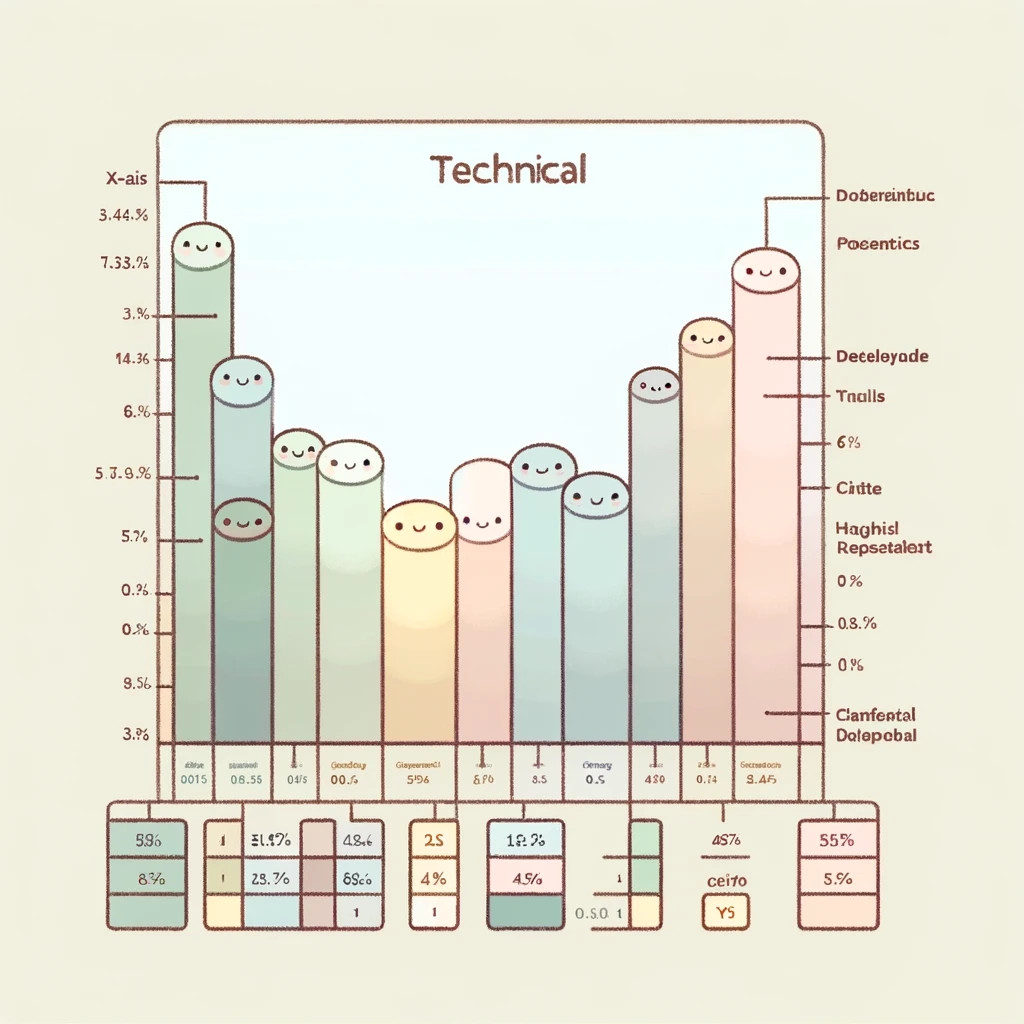
\includegraphics[width=0.45\textwidth]{images/plot.jpg}
    \caption{Plot}
    \label{fig:plot}
\end{figure}

Nam sed tellus id magna elementum tincidunt. Sed ut perspiciatis unde omnis iste natus error sit voluptatem accusantium doloremque laudantium, totam rem aperiam, eaque ipsa quae ab illo inventore veritatis et quasi architecto beatae vitae dicta sunt explicabo. Vestibulum erat nulla, ullamcorper nec, rutrum non, nonummy ac, erat. Nemo enim ipsam voluptatem quia voluptas sit aspernatur aut odit aut fugit, sed quia consequuntur magni dolores eos qui ratione voluptatem sequi nesciunt. Fusce tellus odio, dapibus id fermentum quis, suscipit id erat. Fusce tellus. Nullam rhoncus aliquam metus. Integer rutrum, orci vestibulum ullamcorper ultricies, lacus quam ultricies odio, vitae placerat pede sem sit amet enim. Duis pulvinar. Ut enim ad minima veniam, quis nostrum exercitationem ullam corporis suscipit laboriosam, nisi ut aliquid ex ea commodi consequatur? Nullam faucibus mi quis velit. In dapibus augue non sapien. Etiam dui sem, fermentum vitae, sagittis id, malesuada in, quam.

In laoreet, magna id viverra tincidunt, sem odio bibendum justo, vel imperdiet sapien wisi sed libero. Nunc dapibus tortor vel mi dapibus sollicitudin. Pellentesque sapien. Maecenas aliquet accumsan leo. Curabitur bibendum justo non orci. Nulla quis diam. Integer malesuada. Aliquam erat volutpat. Aliquam ante. Integer rutrum, orci vestibulum ullamcorper ultricies, lacus quam ultricies odio, vitae placerat pede sem sit amet enim. Etiam egestas wisi a erat. Cum sociis natoque penatibus et magnis dis parturient montes, nascetur ridiculus mus. Nullam sit amet magna in magna gravida vehicula. In convallis. Nunc dapibus tortor vel mi dapibus sollicitudin. Proin in tellus sit amet nibh dignissim sagittis. Neque porro quisquam est, qui dolorem ipsum quia dolor sit amet, consectetur, adipisci velit, sed quia non numquam eius modi tempora incidunt ut labore et dolore magnam aliquam quaerat voluptatem.



\section*{Acknowledgment}
Vestibulum erat nulla, ullamcorper nec, rutrum non, nonummy ac, erat. Aliquam erat volutpat. Etiam sapien elit, consequat eget, tristique non, venenatis quis, ante. Maecenas sollicitudin.

\printbibliography

\end{document}
